\section{Reproducibility Summary}

\subsection*{Scope of Reproducibility}
    
We are reproducing \emph{Comparing Rewinding and Fine-tuning in Neural Networks}, by \cite{Renda}.
In this work the authors compare three different approaches to retraining neural networks after pruning: 1) fine-tuning, 2) rewinding weights as in \cite{Frankle} and 3) a new, original method involving learning rate rewinding, building upon \cite{Frankle}. We reproduce the results of all three approaches, but we focus on verifying Renda's original approach: learning rate rewinding, since it is newly proposed and is described as a universal alternative to other methods.

As the authors of \cite {Renda}, we used CIFAR10 for most of the experiments, but we added experiments on a larger version of this dataset: CIFAR100. We have also extended the list of tested network architectures to include Wide ResNets \cite{wrn}. The new experiments led us to discover the limitations of learning rate rewinding which in some cases can worsen pruning results on large neural network architectures.

\subsection*{Methodology}

We implemented the code ourselves in Python with TensorFlow 2, basing our implementation of the paper alone and without consulting the source code provided by the authors. We ran two sets of experiments. In the reproduction set, we have striven to exactly reproduce the experimental conditions of \cite{Renda}. We have also conducted additional experiments, which use other network architectures, effectively showing results previously unreported by the authors. We did not cover all originally reported experiments -- we covered as many as needed to state the validity of claims. We used Google Cloud resources and a local machine with 2x RTX 3080 GPUs.

\subsection*{Results}

We were able to reproduce the exact results reported by the authors in all originally reported scenarios. However, extended results on larger Wide Residual Networks have demonstrated the limitations of the newly proposed learning rate rewinding -- we observed a previously unreported accuracy degradation in low sparsity ranges. Nevertheless, the general conclusion of the paper still holds and was indeed reproduced.

\subsection*{What was easy}

Re-implementation of pruning and retraining methods was technically easy, as it is based on a popular and simple pruning criterion -- magnitude pruning. Original work was descriptive enough to reproduce the results with satisfying results without consulting the code.

\subsection*{What was difficult}

Not every design choice was mentioned in the paper, thus reproducing the exact results was rather difficult and required a meticulous choice of hyper-parameters. Experiments on ImageNet and WMT16 datasets were time consuming and required extensive resources, thus we did not verify them.

% Describe which parts of your reproduction study were difficult or took much more time than you expected. Perhaps the data was not available and you could not verify some experiments, or the author's code was broken and had to be debugged first. Or, perhaps some experiments just take too much time/resources to run and you couldn't verify them. The purpose of this section is to indicate to the reader which parts of the original paper are either difficult to re-use, or require a significant amount of work and resources to verify.

\subsection*{Communication with original authors}

We did not consult the original authors, as there was no need to.

\clearpage

\renewcommand{\arraystretch}{1.5}

\section{Introduction}

Neural network pruning is an algorithm that intends to decrease the size of a network, usually by removing some of its connections or setting their weights to 0. 
This procedure generally allows obtaining smaller and more efficient models.
It often turns out that these smaller networks are as accurate as their bigger counterparts or the accuracy loss is negligible.
A common way to obtain such high quality sparse network is to prune it after the training has finished \cite{Frankle}, \cite{rethinking}.
Networks that have already converged are easier to prune than randomly initialized networks \cite{snip}, \cite{rethinking}.
After pruning, more training is usually required to restore the lost accuracy.
Although there are a few ways to retrain the network, finetuning might be the easiest and most often chosen by researchers and practitioners \cite{Renda}, \cite{rethinking}.

Lottery Ticket Hypothesis from \cite{Frankle} formulates a hypothesis that for every non-pruned neural network, there exists a smaller subnetwork that matches or exceeds results of the original. The algorithm originally used to obtain examples of such networks is iterative magnitude pruning with weight rewinding, and it is one of the three methods of retraining after pruning compared in this work.

\subsection{Structured and Unstructured Pruning}

One of the first papers about neural network pruning \cite{optimal} focused solely on unstructured pruning.
However, current hardware limitations do not allow to take full advantage of this form of pruning.
Structured pruning is a workaround to this problem.
In structured pruning, we remove the basic building blocks of a network instead of single connections.
In the case of dense linear neural networks, these structures are neurons and their connections -- neuron's inputs and outputs.
Depending on the network's type, this can be something else.
In every case, it should be a minimal unit such that the remaining neural network can be represented as a smaller, but still dense (non-pruned) neural network.
In the case of structured pruning of convolutional neural networks, whole channels and their corresponding parameters in convolutional filters are removed.

% A few sentences placing the work in high-level context. Limit it to a few paragraphs at most; your report is on reproducing a piece of work, you don’t have to motivate that work.

\section{Scope of reproducibility}
\label{sec:claims}

% Introduce the specific settings or problem addressed in this work, and list the main claims from the original paper. Think of this as writing out the main contributions of the original paper. Each claim should be relatively concise; some papers may not clearly list their claims, and one must formulate them in terms of the presented experiments. (For those familiar, these claims are roughly the scientific hypotheses evaluated in the original work.)

% A claim should be something that can be supported or rejected by your data. An example is, ``Finetuning pretrained BERT on dataset X will have higher accuracy than an LSTM trained with GloVe embeddings.''
% This is concise, and is something that can be supported by experiments.
% An example of a claim that is too vague, which can't be supported by experiments, is ``Contextual embedding models have shown strong performance on a number of tasks. We will run experiments evaluating two types of contextual embedding models on datasets X, Y, and Z."

% This section roughly tells a reader what to expect in the rest of the report. Clearly itemize the claims you are testing:
Our reproducibility study tries to confirm claims from \cite{Renda}.
Following claims were formulated:
\begin{itemize}
    \item [Claim 1:] Widely used method of training after pruning: finetuning yields worse results than rewinding based methods (supported by figures \ref{fig:resnet20-1}, \ref{fig:resnet56}, \ref{fig:resnet20-2}, \ref{fig:resnet56-2} and Table~\ref{tab:resnet110})
    \item [Claim 2:] Newly introduced learning rate rewinding works as good or better as weight rewinding in all scenarios (supported by figures \ref{fig:resnet20-1}, \ref{fig:resnet56}, \ref{fig:resnet20-2}, \ref{fig:resnet56-2} and Table~\ref{tab:resnet110}, but not supported by Figure~\ref{fig:wrn-1})
    \item [Claim 3:] Iterative pruning with learning rate rewinding matches state-of-the-art pruning methods \\(supported by figures \ref{fig:resnet20-1}, \ref{fig:resnet56}, \ref{fig:resnet20-2}, \ref{fig:resnet56-2} and Table~\ref{tab:resnet110}, but not supported by Figure~\ref{fig:wrn-1})
\end{itemize}

% Each experiment in Section~\ref{sec:results} will support (at least) one of these claims, so a reader of your report should be able to separately understand the \emph{claims} and the \emph{evidence} that supports them.

%\jdcomment{To organizers: I asked my students to connect the main claims and the experiments that supported them. For example, in this list above they could have ``Claim 1, which is supported by Experiment 1 in Figure 1.'' The benefit was that this caused the students to think about what their experiments were showing (as opposed to blindly rerunning each experiment and not considering how it fit into the overall story), but honestly it seemed hard for the students to understand what I was asking for.}

\section{Methodology}
% Explain your approach - did you use the author's code, or did you aim to re-implement the approach from the description in the paper? Summarize the resources (code, documentation, GPUs) that you used.

% Describe how the hyperparameter values were set. If there was a hyperparameter search done, be sure to include the range of hyperparameters searched over, the method used to search (e.g. manual search, random search, Bayesian optimization, etc.), and the best hyperparameters found. Include the number of total experiments (e.g. hyperparameter trials). You can also include all results from that search (not just the best-found results).

We aimed to compare three retraining approaches: 1) finetuning, 2) weight rewinding and 3) learning rate rewinding. Our general strategy that repeated across all experiments was as follows:
\begin{enumerate}
    \item train a neural network to convergence,
    \item prune the network using magnitude criterion: remove parameters with the smallest absolute value,
    \item retrain the network using one of the three retraining approaches.
\end{enumerate}

In the case of structured pruning: in step 2, we removed structures (either neurons or convolutional channels) with the smallest L1 norm \cite{structured}, rather than removing separate connections. 

In the case of iterative pruning: the network in step 1 was not randomly initialized, but instead: weights from a model from a previous iterative pruning step were loaded as the starting point.
Then the three steps were repeated.
On the other hand, one-shot pruning is a procedure where pruning is done only once, so there was only one cycle.
In some methods, this might be done on a randomly initialized neural network, like in \cite{snip}.
Here, however, one-shot pruning is done after the network reaches convergence.
So the three steps are not repeated in case of one-shot pruning.

We trained all our networks using Stochastic Gradient Descent with Nesterov Momentum \cite{nesterov}. The learning rate was decreased in a piecewise manner during the training, but momentum coefficient was constant and equal to $0.9$.

\section{Model descriptions}

In this report, we were focusing on an image recognition task using convolutional neural networks \cite{lecun_convnet}. 
For most of our experiments, we chose to use identical architectures as \cite{Renda} to better validate their claims and double-check their results, rather than only provide additional ones.
Therefore, most of the used networks are residual networks, which were originally proposed in \cite{resnet}.
Additionally, to verify the general usefulness of pruning and retraining methods proposed in \cite{Renda} we extend the list of tested network architectures to much larger wide residual networks from \cite{wrn}.

\subsection{Residual networks (ResNet)}

Just as \cite{Renda}, we chose to use the original version of ResNet as described in \cite{resnet} rather than the more widely used, improved version (with preactivated blocks) from \cite{resnetv2}. We created the models ourselves, using TensorFlow \cite{tensorflow} and Keras. We strove to replicate the exact architectures used by \cite{Renda} and \cite{resnet} and train them from scratch.

\begin{table}[H]
\small
\setlength{\tabcolsep}{10pt}
  \begin{center}
    \begin{tabular}{l|c|c|c|c}
      \specialrule{1pt}{2pt}{2pt}
    \textbf{Model} & \textbf{Trainable parameters} & \textbf{Kernel parameters} & \textbf{CIFAR-10} & \textbf{CIFAR-100} \\ 
      \specialrule{0.5pt}{2pt}{2pt}
      ResNet-20  & \numprint{272282} & \numprint{270896} & 92.46\% & -- \\
      ResNet-56  & \numprint{855578} & \numprint{851504} & 93.71\% & 71.90\% \\
      ResNet-110 & \numprint{1730522} & \numprint{1722416} & 94.29\% & 72.21\% \\
      \specialrule{0.5pt}{2pt}{2pt}
    \end{tabular}
  \end{center}
\caption{ResNets architecture summary, including baseline accuracy across datasets.}
\label{tab:resnet}
\end{table}

% GOOD PLACE TO INSERT MERMAID DIAGRAM TO SHOW DIFFERENCES BETWEEN v1 and v2 ResNets

\subsubsection{ResNet hyperparameters}

% \nopagebreak
Learning rate started with $0.1$ and was multiplied by $0.1$ twice, after \numprint{36000} and \numprint{54000} iterations. One training cycle had \numprint{72000} iterations in total.
For all batch normalization layers, we set the batch norm decay to 0.997, following \cite{Renda}, which is also the default used in the original TensorFlow implementation\footnote{\url{https://github.com/tensorflow/models/blob/r1.13.0/official/resnet/resnet_model.py}}.
We initialize network's weights with what is known as He uniform initialization from \cite{he_uniform}.
We regularize ResNets, during both training and finetuning, using $L2$ penalty with $10^{-4}$ coefficient.
In other words, the loss function (from which we calculate the gradients) looks as follows:

\begin{equation}
  L = \textup{CC}(y, p) + 10^{-4} \times \sum_{i\in W} w_i^2
  \end{equation}
  where:
  \begin{conditions}
   L     &  value of the final loss function \\
   \textup{CC}    &  categorical crossentropy loss function \\
   y     &  ground truth label of a sample or batch \\   
   p &  model's prediction \\
   W & parameters of the model
  \end{conditions}

\subsection{Wide Residual Networks (Wide ResNet, WRN)}

WRN networks were introduced in \cite{wrn}.
They are residual networks created by simply increasing the number of filters in preactivated ResNet networks \cite{resnetv2}.

\begin{table}[H]
\small
\setlength{\tabcolsep}{12pt}
  \begin{center}
    \begin{tabular}{l|c|c|c}
      \specialrule{1pt}{2pt}{2pt}
      \textbf{Model} & \textbf{Trainable parameters} & \textbf{Kernel parameters} & \textbf{CIFAR-10}\\ 
      \specialrule{0.75pt}{2pt}{2pt}
      WRN-16-8 & \numprint{10961370} & \numprint{10954160} & 95.72\% \\
      \specialrule{0.75pt}{2pt}{2pt}
    \end{tabular}
  \end{center}
\caption{Wide ResNet architecture summary.}\label{tab:wrn}
\end{table}
% Include a description of each model or algorithm used. Be sure to list the type of model, the number of parameters, and other relevant info (e.g. if it's pretrained). 

\subsubsection{WRN hyperparameters}

\nopagebreak
As Wide ResNets are newer and much larger than ResNets, hyper-parameters are slightly different.
To choose them, we follow \cite{wrn}. Learning rate starts with $0.1$ and multiplied by $0.2$ thrice: after \numprint{32000}, \numprint{48000} and \numprint{64000} iterations. Training lasts for \numprint{80000} iterations. For all batch normalization layers, we use hyper-parameters from the newer TensorFlow implementation\footnote{\url{https://github.com/tensorflow/models/blob/r2.5.0/official/vision/image_classification/resnet/resnet_model.py}} with batch norm decay set to 0.9. Following \cite{wrn}, we use larger $L2$ penalty for this network: $2\times10^{-4}$. Finally, the loss function is as follows:

\begin{equation}
  L = \textup{CC}(y, p) + 2 \times 10^{-4} \times \sum_{i\in W} w_i^2
  \end{equation}
  where:
  \begin{conditions}
   L     &  value of the final loss function \\
   \textup{CC}    &  categorical crossentropy loss function \\
   y     &  ground truth label of a sample or batch \\   
   p &  model's prediction \\
   W & parameters of the model
  \end{conditions}

\subsection{Datasets}

CIFAR-10 and CIFAR-100 are image classification datasets introduced in \cite{cifar10}. Following \cite{Renda}, we use all (\numprint{50000}) training examples to train the model.

\begin{table}[H]
\small
\setlength{\tabcolsep}{6pt}
  \begin{center}
    \begin{tabular}{l|c|c|c|c}
      \specialrule{1pt}{2pt}{2pt}
\textbf{Dataset} & \textbf{Training examples} & \textbf{Validation examples} & \textbf{Classes} & \textbf{Resolution}\\ 
      \specialrule{0.5pt}{2pt}{2pt}
      CIFAR-10  & \numprint{50000} & \numprint{10000} & 10 & 32$\times$32\\
      CIFAR-100  & \numprint{50000} & \numprint{10000} & 100 & 32$\times$32\\
      \specialrule{0.5pt}{2pt}{2pt}
    \end{tabular}
  \end{center}
\caption{CIFAR datasets description.}\label{tab:cifar}
\end{table}

\subsection{Preprocessing and data augmentation}
We used a standard data processing for both CIFAR-10 and CIFAR-100 datasets \cite{Renda}, \cite{Frankle}, \cite{wrn}. During training and just before passing data to the model, we:
\begin{enumerate}
    \item standardized the input by subtracting the mean and dividing by the std of RGB channels (calculated on training dataset),
    \item randomly flipped in horizontal axis,
    \item added a four pixel reflection padding,
    \item randomly cropped the image to its original resolution.
\end{enumerate}

During the validation, we did only the first step of the above.

% For each dataset include 1) relevant statistics such as the number of examples and label distributions, 2) details of train / dev / test splits, 3) an explanation of any preprocessing done, and 4) a link to download the data (if available).


\subsection{Experimental setup and code}
% Include a description of how the experiments were set up that's clear enough a reader could replicate the setup. 
% Include a description of the specific measure used to evaluate the experiments (e.g. accuracy, precision@K, BLEU score, etc.). 
% Provide a link to your code.


Our ready-to-use code, which includes experiment definitions, can be found at 
% \url{https://anonymous.4open.science/r/reproducing-comparing-rewinding-and-finetuning-1C5A}.
\url{https://github.com/gahaalt/reproducing-comparing-rewinding-and-finetuning}.
It's written using TensorFlow \cite{tensorflow} version 2.4.2 in Python. More details are included in the repository.

\subsection{Computational requirements}
% Include a description of the hardware used, such as the GPU or CPU the experiments were run on. 
% For each model, include a measure of the average runtime (e.g. average time to predict labels for a given validation set with a particular batch size).
% For each experiment, include the total computational requirements (e.g. the total GPU hours spent).
% (Note: you'll likely have to record this as you run your experiments, so it's better to think about it ahead of time). Generally, consider the perspective of a reader who wants to use the approach described in the paper --- list what they would find useful.

Recreating the experiments required a modern GPU, training all models on CPU was virtually impossible. Training time varies depending on a lot of factors: network variation and size, exact version of the deep learning library, and even the operating system. In our case, using TensorFlow 2.4.2 on Ubuntu and a single RTX 3080 GPU, the smallest of the used models, ResNet-20, takes about 20 minutes to train on CIFAR-10 dataset. To replicate our experiments, training at least a single baseline network and then, once more, a single pruned network, is required. To reduce computational requirements, we reused one non-pruned baseline for multiple compression ratios. Approximated training time requirements can be seen in the table below.

\begin{table}[H]
\small
\setlength{\tabcolsep}{6pt}
  \begin{center}
    \begin{tabular}{l|c|c|c|c}
      \specialrule{1pt}{2pt}{2pt}
\textbf{Model} & \textbf{Dataset} & \textbf{Number of updates} & \textbf{Updates per second} & \textbf{Training time}\\ 
      \specialrule{0.5pt}{2pt}{2pt}
      ResNet-20  & CIFAR-10 & \numprint{72000} & 59.0 & 22 min \\
      ResNet-56  & CIFAR-10 & \numprint{72000} & 28.6 & 43 min \\
      ResNet-110  & CIFAR-10 & \numprint{72000} & 15.9 & 77 min \\
      WRN-16-8  & CIFAR-10 & \numprint{80000} & 17.4 & 78 min \\
      \specialrule{0.5pt}{2pt}{2pt}
    \end{tabular}
  \end{center}
\caption{Time requirements for replicating or running experiments from this report. Reported times are obtained using a single RTX 3080 GPU in Linux environment, using TensorFlow in version 2.4.2.}
\label{tab:compute}
\end{table}

For all our experiments together, we estimate the total number of GPU hours spent to be around 540.

\section{Method description}

% Start with a high-level overview of your results. Do your results support the main claims of the original paper? Keep this section as factual and precise as possible, reserve your judgement and discussion points for the next "Discussion" section. 

We compare three methods of retraining after pruning. For all of them, the starting point is a network that was already trained to convergence, then pruned to a desired sparsity. The difference between the three retraining methods is what follows after it.

\subsection{Fine-tuning}
Fine-tuning is retraining with a small, constant learning rate -- in our case, whenever fine-tuning was used, the learning rate was set to 0.001 as in \cite{Renda}. We finetune the network for the same number of iterations as the baseline -- \numprint{72000} iterations in the case of the original ResNet architecture. In this method, such long retraining would not be necessary in practical applications, since the network converges much faster.

\subsection{Weight rewinding}
Weight rewinding restores the network's weights from a previous point (possibly beginning) in the training history and then continues training from this point using the original training schedule -- in our case a piecewise constant decaying learning rate schedule.
When rewinding a network to iteration $K$ that originally trained for $N$ iterations: first prune the non-pruned network that was trained for $N$ iterations. Then, for connections that survived, restore their values to $K$-th iteration from the training history. Then train to the convergence for the remaining $N-K$ iterations.

\subsection{Learning rate rewinding}
Learning rate rewinding continues training with weights that have already converged, but restores the learning rate schedule to the beginning, just as if we were training from scratch, and then trains to the convergence once again. This reminds the cyclical learning rates from \cite{cyclical}. Learning rate rewinding really is weight rewinding for $K = N$, but the final retraining is always for $N$ iterations.

\section{Results reproducing original paper}
In most of our experiment, just as \cite{Renda}, we investigate how does the trade-off between prediction accuracy and compression ratio look like. 
In one of the experiments (Table~\ref{tab:resnet110}) we verify only one compression ratio, but for the rest, we verify multiple.
We report a median result out of 2 up to 12 trials for each compression ratio. To better utilize our compute capabilities, we decided to spend more training cycles in situations where there is no clear winner between the compared methods. On each plot, we include error bars showing 80\% confidence intervals.

In this section, we include experiments that we successfully reproduced.
Most of them match the original ones within 1\% error margin.
We noticed some of our results were slightly better than authors of \cite{Renda} originally reported.


Across all scenarios where finetuning was tested, it was by far the worst of the three methods, which directly supports claim 1 (Section~\ref{sec:claims}). Weight rewinding and learning rate rewinding most often are equally matched, but in some cases learning rate rewinding works a little better.

\subsection{ResNets on CIFAR-10 dataset}

\nopagebreak

Results we observe here are consistent with what we see in \cite{Renda}, \cite{Frankle}.
Iterative pruning is better than one-shot pruning, but more time consuming.
In extreme cases, iterative pruning requires 20 times as many iterations than one-shot pruning to complete.
But it is not as bad for moderate sparsity pruning.
Larger networks work better than smaller ones.
Even when the number of parameters left after pruning is the same -- originally larger network will outperform the smaller one.

Out of the retraining methods, weight rewinding and learning rate rewinding seem to be similar, but finetuning is visibly worse.
In some cases, learning rate rewinding outperforms weight rewinding.
Similar conclusions can be drawn from both structured and unstructured pruning results.

\begin{figure}[H]
  \setlength{\tabcolsep}{0pt}
  \centering
      \begin{tabular}{c}
        \includegraphics[width=0.7\linewidth]{pics/Resnet20-structured.pdf}
      \end{tabular}
  \caption{Results of ResNet-20 (Table~\ref{tab:resnet}) on CIFAR-10 (Table~\ref{tab:cifar}) with structured, one-shot, magnitude pruning. Results show varying compression ratios. Maximal compression ratio (9.35$\times$) means that there are only \numprint{29000} non-zero kernel parameters left in ResNet-20.}
  \label{fig:resnet20-2}
  \end{figure}

\begin{figure}[H]
\centering
\setlength{\tabcolsep}{0pt}
\begin{tabular}{c}
\includegraphics[width=1.0\linewidth]{pics/Resnet20-1s-iterative.pdf}
\end{tabular}
\caption{Results of ResNet-20 (Table~\ref{tab:resnet}) on CIFAR-10 (Table~\ref{tab:cifar}) with unstructured, magnitude pruning in versions: one-shot and iterative. Results show varying compression ratios. Maximal compression ratio (9.35$\times$) means that there are only \numprint{29000} non-zero kernel parameters left. This experiment supports claims 1, 2, 3 (Section~\ref{sec:claims}).}
\label{fig:resnet20-1}
\end{figure}

\begin{figure}[H]
\setlength{\tabcolsep}{0pt}
\centering
    \begin{tabular}{c}
      \includegraphics[width=1.0\linewidth]{pics/Resnet56-1s-iterative.pdf}
    \end{tabular}
\caption{Results of ResNet-56 (Table~\ref{tab:resnet}) on CIFAR-10 (Table~\ref{tab:cifar}) with unstructured, magnitude pruning in versions: one-shot and iterative. Results with varying compression ratios. Maximal compression ratio means (22.73$\times$) that there are only \numprint{37600} non-zero kernel parameters left. This experiment supports claims 1, 2, 3 (Section~\ref{sec:claims}).}
\label{fig:resnet56}
\end{figure}

\begin{table}[H]
\small
\setlength{\tabcolsep}{14pt}
  \begin{center}
    \begin{tabular}{l|c|c|c|c}
      \specialrule{1pt}{2pt}{2pt}
\textbf{Network} & \textbf{Dataset} & \textbf{Retraining} & \textbf{Sparsity} & \textbf{Test Accuracy} \\ 
      \specialrule{0.75pt}{2pt}{2pt}
      ResNet-110  & CIFAR-10 & None & 0\% & 94.29\% \\
      ResNet-110  & CIFAR-10 & LR rewinding & 89.3\% & 93.74\% \\
      ResNet-110  & CIFAR-10 & weight rewinding & 89.3\% & 93.73\% \\
      ResNet-110  & CIFAR-10 & finetuning & 89.3\% & 93.32\% \\
      \specialrule{0.75pt}{2pt}{2pt}
    \end{tabular}
  \end{center}
\caption{Results of ResNet-110 (Table~\ref{tab:resnet}) trained on CIFAR-10 (Table~\ref{tab:cifar}) with unstructured, one-shot magnitude pruning. Sparsity $89.3\%$ corresponds to $9.35\times$ compression ratio. This experiment supports claims 1, 2, 3 (Section~\ref{sec:claims}).}
\label{tab:resnet110}
\end{table}




% \begin{center}
% \begin{tabular}{cc} 
% \rotatebox[origin=c]{90}{CIFAR-10} &  \\
%  \hline
%  \rotatebox[origin=c]{90}{CIFAR-100} & \includegraphics[width=0.8\linewidth]{Resnet20vsResnet50} \\
% \end{tabular}
% \end{center}


% For each experiment, say 1) which claim in Section~\ref{sec:claims} it supports, and 2) if it successfully reproduced the associated experiment in the original paper. 
% For example, an experiment training and evaluating a model on a dataset may support a claim that that model outperforms some baseline.
% Logically group related results into sections. 


\section{Results beyond original paper}
% Often papers don't include enough information to fully specify their experiments, so some additional experimentation may be necessary. For example, it might be the case that batch size was not specified, and so different batch sizes need to be evaluated to reproduce the original results. Include the results of any additional experiments here. Note: this won't be necessary for all reproductions.
 
\subsection{ResNets on CIFAR-100 dataset}
\nopagebreak
\begin{figure}[H]
\setlength{\tabcolsep}{0pt}
\centering
    \begin{tabular}{c}
      \includegraphics[width=0.7\linewidth]{pics/Resnet56-C100.pdf}
    \end{tabular}
\caption{Results of ResNet-56 (Table~\ref{tab:resnet}) on CIFAR-100 (Table~\ref{tab:cifar}) with unstructured, one-shot, magnitude pruning. Results with varying compression ratios. Maximal compression ratio (9.35$\times$) means that there are only \numprint{91500} non-zero kernel parameters left. This experiment supports claims 1, 2, 3 (Section~\ref{sec:claims}) even though this scenario wasn't originally tested in \cite{Renda}.}
\label{fig:resnet56-2}
\end{figure}

\subsection{WRN-16-8 on CIFAR-10 dataset}
\nopagebreak

WRN-16-8 shows consistent behaviour -- accuracy in the low sparsity regime is reduced in comparison to the baseline. In the case of iterative pruning, where each step is another pruning in the low sparsity regime, it leads to a large difference between the two retraining methods. Since for WRN-16-8 one-shot, low sparsity pruning shows a small accuracy regression in comparison to the baseline, this regression accumulates when pruning multiple times, which we do in iterative pruning. We think that the degradation we observe in the case of iterative pruning is an effect of stacking multiple smaller defects that we observe in the case of one-shot pruning. This can be seen in Figure~\ref{fig:wrn-1}.

\begin{figure}[H]
\setlength{\tabcolsep}{0pt}
  \begin{center}
    \begin{tabular}{c}
      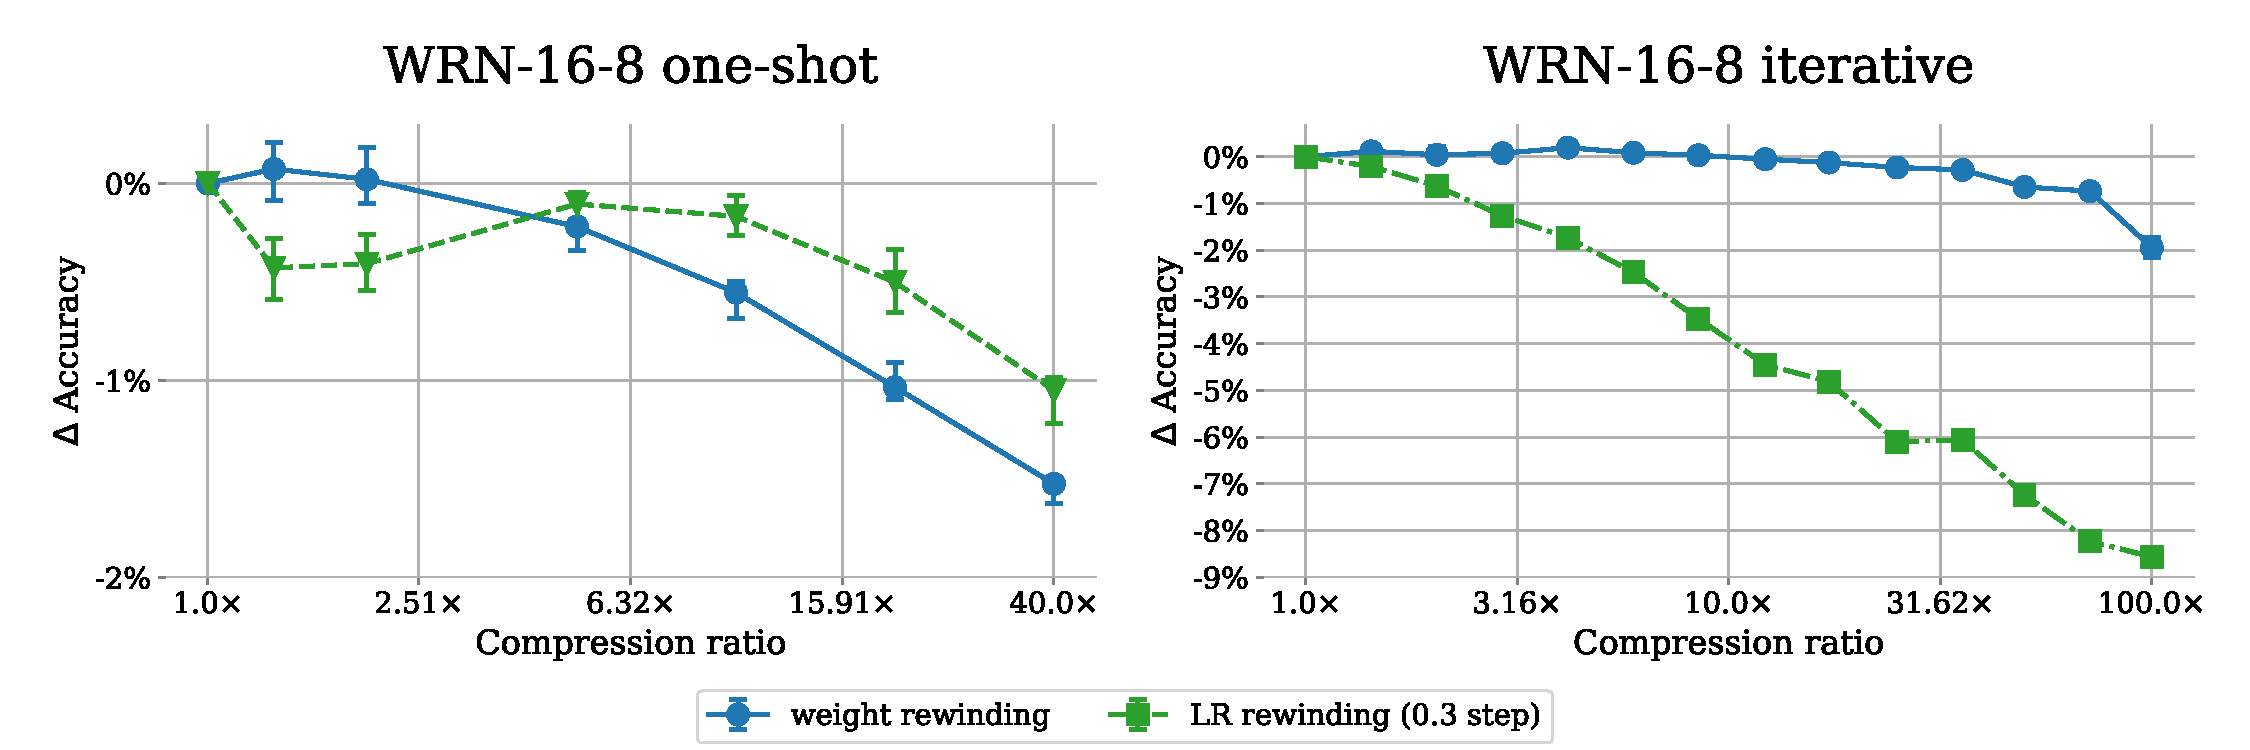
\includegraphics[width=1.0\linewidth]{pics/WRN-16-8-LR-rewinding-is-flawed2.pdf}\\
    \end{tabular}
  \end{center}
\caption{Results of WRN-16-8 (Table~\ref{tab:wrn}) on CIFAR-10 (Table~\ref{tab:cifar}) with unstructured, magnitude pruning in versions: one-shot and iterative. Results with varying compression ratios. Maximal compression ratio (100$\times$) leaves \numprint{109500} non-zero kernel parameters while achieving around 94\% accuracy or around 95\% when leaving \numprint{153400} non-zero parameters. One can see catastrophic effects of high-sparsity pruning when using learning rate rewinding procedure.}
\label{fig:wrn-1}
\end{figure}

For iterative pruning (figures \ref{fig:resnet20-1}, \ref{fig:resnet56}, \ref{fig:wrn-1}) we used a nonstandard step size of 30\% per iterative pruning iteration, which was a way to reduce the computational requirements. We believe this choice does not change the validity of the claims, and to support it, we provide a comparison of our step size to the more commonly used 20\%. We show that there is virtually no difference between both versions and the aforementioned catastrophic degradation occurs in both cases, as long as the step size is in the low sparsity regime.

\begin{figure}[H]
\setlength{\tabcolsep}{0pt}
  \begin{center}
    \begin{tabular}{c}
      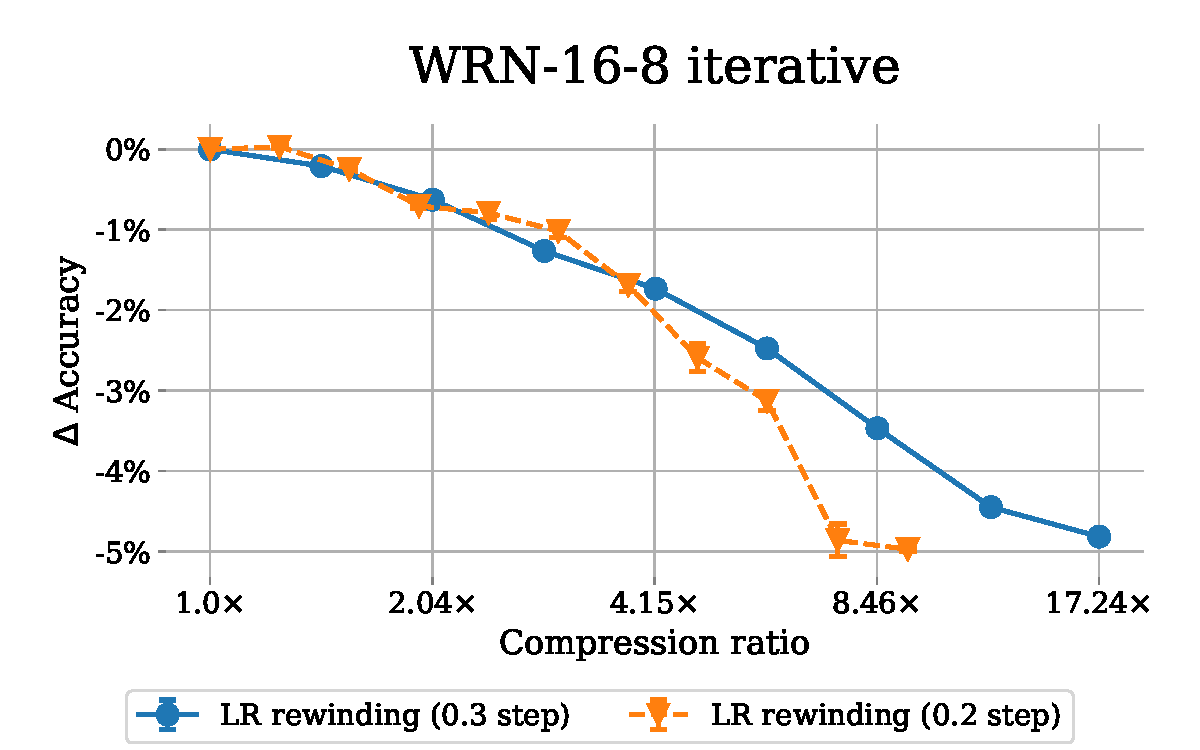
\includegraphics[width=0.7\linewidth]{pics/WRN-16-8-LR-rew-compare2v3.pdf}\\
    \end{tabular}
  \end{center}
\caption{Results of WRN-16-8 (Table~\ref{tab:wrn}) on CIFAR-10 (Table~\ref{tab:cifar}) with unstructured, iterative, magnitude pruning with two different step sizes. Results show varying compression ratios and accuracy.}
\label{fig:wrn-2}
\end{figure}

\section{Discussion}

We were able to confirm the general conclusion of \cite{Renda}. Fine-tuning can be mostly replaced by other retraining techniques, e.g., by weight rewinding as it was done by \cite{Frankle}. We confirmed that learning rate rewinding worked even better in some scenarios. However, we have also shown in Figure~\ref{fig:wrn-1} that the newly proposed learning rate rewinding is a poor choice when we are pruning large networks -- in our case that is WRN-16-8. We believe this should be examined further as there might exist a simple workaround to this problem -- a retraining procedure between weight rewinding and learning rate rewinding, which works even for larger networks. Furthermore, it would be interesting to see what happens in the network when this catastrophic accuracy degradation occurs. Perhaps, the reason for it not occurring with the original ResNet, but occurring with larger architectures, is the degree to which the larger networks overtrain -- larger networks tend to overfit more. And such an overfitted network might be not a good starting point for the retraining.

% Give your judgement on if your experimental results support the claims of the paper. Discuss the strengths and weaknesses of your approach - perhaps you didn't have time to run all the experiments, or perhaps you did additional experiments that further strengthened the claims in the paper.

\section*{Acknowledgements}
The authors thank Polish National Science Center for funding
under the OPUS-18 \linebreak[4] 2019/35/B/ST6/04379 grant and the PlGrid
consortium for computational resources.
